\documentclass[a4paper,11pt,oneside]{amsbook}

\usepackage[rgb]{xcolor}
\usepackage{comments}
\usepackage{booktabs}
\usepackage[T1]{fontenc}
\usepackage{lmodern}
\usepackage{microtype}
\usepackage{amssymb}
\usepackage{amsrefs}
\usepackage{enumitem}
\usepackage{graphicx}
\usepackage{subcaption}
\usepackage{pdfpages}
\usepackage{hyperref}
\usepackage[capitalise,noabbrev]{cleveref}
\usepackage{etoolbox}
\usepackage{pgfkeys}
\usepackage{minted}
\usepackage{tikz}
\usepackage{newfloat}
\usepackage[noend,noline,linesnumbered]{algorithm2e}
\usepackage{xparse}
\usepackage{chngcntr}
\usepackage{lipsum}

%\usepackage{showframe}

% less aggressive hyperlinks
\hypersetup{%
  pdfborderstyle={/S/U/W 1}, % underline links instead of boxes
  linkbordercolor=red,       % color of internal links
  citebordercolor=green,     % color of links to bibliography
  filebordercolor=magenta,   % color of file links
  urlbordercolor=cyan        % color of external links
}
% since I refer to listings across sections
\counterwithin{listing}{section}
\counterwithin{figure}{section}

% tikz setup
\usetikzlibrary{arrows,fit,positioning,matrix,calc,scopes,chains,tikzmark}

% example environment
\newtheorem{example}{Example}[section]

% temporal operators
\makeatletter
\input pdf-trans
\newbox\qbox
\def\usecolor#1{\csname\string\color@#1\endcsname\space}
\newcommand\outline[1]{\leavevmode%
  \def\maltext{#1}%
  \setbox\qbox=\hbox{\maltext}%
  \boxgs{Q q 2 Tr .3\space w \fillcol\space \bordercol\space}{}%
  \copy\qbox%
}
\makeatother

\newcommand\colsplit[2]{\colorlet{tmpcolor}{#2}\edef\tmp{\usecolor{tmpcolor}}%
  \def\tmpB{}\expandafter\colsplithelp\tmp\relax%
  \ifnum0=#1\relax\edef\fillcol{\tmpB}\else\edef\bordercol{\tmpC}\fi}
\def\colsplithelp#1#2 #3\relax{%
  \edef\tmpB{\tmpB#1#2 }%
  \ifnum `#1>`9\relax\def\tmpC{#3}\else\colsplithelp#3\relax\fi
}
\colsplit{1}{black}
\colsplit{0}{white}

\DeclareFontFamily{U}{mathb}{\hyphenchar\font45}
\DeclareFontShape{U}{mathb}{m}{n}{
      <5> <6> <7> <8> <9> <10> gen * mathb
      <10.95> mathb10 <12> <14.4> <17.28> <20.74> <24.88> mathb12
      }{}
\DeclareSymbolFont{mathb}{U}{mathb}{m}{n}

\DeclareFontFamily{U}{matha}{\hyphenchar\font45}
\DeclareFontShape{U}{matha}{m}{n}{
      <5> <6> <7> <8> <9> <10> gen * matha
      <10.95> matha10 <12> <14.4> <17.28> <20.74> <24.88> matha12
      }{}
\DeclareSymbolFont{matha}{U}{matha}{m}{n}

\makeatletter
\newcommand{\superimpose}[2]{%
  {\ooalign{$#1\@firstoftwo#2$\cr\hfil$#1\@secondoftwo#2$\hfil\cr}}}
\newcommand{\raisemath}[1]{\mathpalette{\raisem@th{#1}}}
\makeatother

\DeclareMathSymbol{\nextP}{\mathbin}{matha}{"0D}
\DeclareMathSymbol{\nextF}{\mathbin}{matha}{"05}
\newcommand{\nextWP}{\mathbin{\hat{\nextP}}}
\newcommand{\nextWF}{\mathbin{\hat{\nextF}}}
\DeclareMathSymbol{\alwaysPP}{\mathbin}{mathb}{"0D}
\newcommand{\alwaysP}{\mathbin{\mathpalette\superimpose{{\alwaysPP}{\alwaysF}}}}
\DeclareMathSymbol{\alwaysF}{\mathbin}{mathb}{"05}
\DeclareMathSymbol{\eventuallyPP}{\mathbin}{mathb}{"0C}
\newcommand{\eventuallyP}{\mathbin{\mathpalette\superimpose{{\eventuallyPP}{\eventuallyF}}}}
\DeclareMathSymbol{\eventuallyF}{\mathbin}{matha}{"0C}
\newcommand{\triggerP}{\mathbin{\mathpalette\superimpose{{\alwaysP}{\textcolor{white}{\cdot}}}}}
\newcommand{\triggerF}{\mathbin{\mathpalette\superimpose{{\alwaysF}{\cdot}}}}
\newcommand{\sinceF}{\mathbin{\mathpalette\superimpose{{\eventuallyF}{\cdot}}}}
\newcommand{\sinceP}{\mathbin{\mathpalette\superimpose{{\eventuallyP}{\textcolor{white}{\cdot}}}}}
\newcommand{\initialP}{\mbox{\bfseries\sffamily I}}
\newcommand{\initialF}{\outline{\bfseries\sffamily F}}
\newcommand\initiallyNP{{\hat{\eventuallyP}}}
\newcommand\initiallyP[1]{{\hat{\eventuallyP} #1}}
\newcommand\initiallyNF{{\hat{\eventuallyF}}}
\newcommand\initiallyF[1]{{\hat{\eventuallyF} #1}}

% breaks in align environment
\newenvironment{alignbr*}{\allowdisplaybreaks\csname align*\endcsname}{\csname endalign*\endcsname}

% operations on states in multi-shot section
\newenvironment{StateOp}{%
\newcommand\opitem[1]{%
\renewcommand\makelabel[1]{####1}
\item[##1]\leavevmode\\}
\description[font=\normalfont,leftmargin=2em]}{%
\enddescription}

% restyle algorithm environment
% (makes it look similar to the listings environment)
\DontPrintSemicolon
\SetStartEndCondition{ }{}{}%
\SetKwComment{tcp}{\#~}{}
\SetKwProg{Fn}{function}{:}{end}
\SetKw{KwTo}{in}
\SetKwFor{For}{for}{\string:}{}%
\SetKwIF{If}{ElseIf}{Else}{if}{:}{else if}{else:}{}%
\SetKwFor{While}{while}{:}{fintq}%
\SetKwFor{ForEach}{for each}{:}{fintq}%
\AlgoDontDisplayBlockMarkers\SetAlgoNoEnd\SetAlgoNoLine%
\setlength{\algomargin}{\leftskip}
\addtolength{\algomargin}{\parskip}
\SetNlSkip{1em}
\SetNlSty{}{}{}
\let\savedalgorithm\algorithm
\let\savedendalgorithm\endalgorithm
\newenvironment{algorithm2e}{%
\renewenvironment{algocf}[1][h]{}{}%
\savedalgorithm}{%
\savedendalgorithm}
\DeclareFloatingEnvironment[name=Algorithm]{algorithmf}
\renewenvironment{algorithm}{%
\algorithmf\raggedright}{%
\endalgorithmf}
\Crefname{algorithmf}{Algorithm}{Algorithms}
\Crefname{algocfline}{Line}{Lines}

% support for nested listings
\DeclareCaptionSubType{listing}
\captionsetup[sublisting]{labelformat=parens}
\Crefname{sublisting}{Listing}{Listings}

\renewcommand{\thesection}{\thechapter.\arabic{section}}
\makeatletter
\def\@seccntformat#1{%
  \protect\textup{\protect\@secnumfont
    \csname the#1\endcsname\enspace
  }%
}
\renewcommand{\tocsection}[3]{%
  \indentlabel{\@ifnotempty{#2}{\ignorespaces#1 #2\quad}}#3}
\makeatother

\newsavebox{\mintedbox}
\NewDocumentEnvironment{mintedsubcaptionbox}{O{#2}mO{}m}{%
  \VerbatimEnvironment%
  \RecustomVerbatimEnvironment{Verbatim}{BVerbatim}{}%
  \begin{lrbox}{\mintedbox}%
  \begin{minted}[escapeinside=||,#3]{#4}}{%
  \end{minted}%
  \end{lrbox}%
  \subcaptionbox[#1]{#2}[.5\linewidth]{\usebox{\mintedbox}}}

\newcommand\inputmintedsubcaptionbox[3]{%
  \RecustomVerbatimEnvironment{Verbatim}{BVerbatim}{}%
  \begin{lrbox}{\mintedbox}%
  \inputminted[escapeinside=\%\#]{#2}{#3}%
  \end{lrbox}%
  \subcaptionbox{#1}[.49\linewidth]{\usebox{\mintedbox}}}

% line refs with the minted package
\newcommand\llabel[1]{\label[line]{#1}\hypertarget{#1}{}}
\newcommand\Lref[1]{Line~\hyperlink{#1}{\ref*{#1}}}
\newcommand\lref[1]{\Lref{#1}}
\newcommand\Lrefrange[2]{Lines~\hyperlink{#1}{\ref*{#1}} to~\hyperlink{#2}{\ref*{#2}}}
\newcommand\lrefrange[2]{\Lrefrange{#1}{#2}}

\makeatletter
\newcounter{lrefs@count}%
\newcounter{lrefs@step}%
\newcommand\lrefs[1]{{%
  \def\lrefs@list{}%
  \forcsvlist{\listadd\lrefs@list}{#1}%
  \setcounter{lrefs@count}{0}%
  \setcounter{lrefs@step}{0}%
  \def\do##1{\stepcounter{lrefs@count}}%
  \dolistloop{\lrefs@list}%
  \def\do##1{%
    \stepcounter{lrefs@step}%
    \ifnum\value{lrefs@step}=1%
      \def\lrefs@pre{Lines~}%
    \else%
      \ifnum\value{lrefs@step}=\value{lrefs@count}%
        \ifnum\value{lrefs@count}=2%
          \def\lrefs@pre{ and~}%
        \else%
          \def\lrefs@pre{, and~}%
        \fi%
      \else%
        \def\lrefs@pre{,~}%
      \fi%
    \fi%
    \lrefs@pre\hyperlink{##1}{\ref*{##1}}%
  }%
  \dolistloop{\lrefs@list}%
}}
\makeatother

% shortcuts for inline Python and ASP code
\newcommand\ASP{\mintinline[escapeinside=||]{clingo}}
\newcommand\Python{\mintinline[breaklines]{python}}

% wrap longer intertext in a parbox
\makeatletter
\newlength{\longintertext@parindent}
\AtBeginDocument{\setlength{\longintertext@parindent}{\parindent}}
\newcommand{\longintertext}[1]{%
  \intertext{%
    \parbox{\linewidth}{%
      \setlength{\parindent}{\longintertext@parindent}
      \noindent#1%
    }%
  }%
}
\makeatother

% macros to include publications
\makeatletter
\pgfkeys{/includepub/.cd,
  title/.initial=,
  label/.initial=,
  path/.initial=,
  authors/.initial=,
  published_in/.initial=,
  bibentry/.initial=,
  url/.code={\pgfkeyssetvalue{includepub@url}{#1}\pgfkeysgetvalue{includepub@url}{\includepub@url}},
  doi/.code={\pgfkeyssetvalue{includepub@doi}{#1}\pgfkeysgetvalue{includepub@doi}{\includepub@doi}},
  note/.code={\pgfkeyssetvalue{includepub@note}{#1}\pgfkeysgetvalue{includepub@note}{\includepub@note}}}

\newcommand\includepub@get[1]{%
  \pgfkeysvalueof{/includepub/#1}}

\newcommand\includepub@include[1]{%
  \ifdef{\Final}%
    {\includepdf[pages=-]{#1}}%
    {\includepdf[pages=1]{#1}}}

\newcommand\includepub[1]{%
  \bgroup%

  \pgfkeys{/includepub/.cd,#1}
  \clearpage
  \section{\includepub@get{title}}\label{\includepub@get{label}}
  \begin{description}
    \item[Authors] \includepub@get{authors}
    \item[Published in] \includepub@get{published_in}
    \item[Bibliography entry] \includepub@get{bibentry}
    \pgfkeysifdefined{includepub@url}
      {\item[URL] \url{\includepub@url}}
      {}
    \pgfkeysifdefined{includepub@doi}
      {\item[DOI] \href{https://doi.org/\includepub@doi}{\includepub@doi}}
      {}
    \pgfkeysifdefined{includepub@note}
      {\item[Notes] \includepub@note}
      {}
  \end{description}
  \includepub@include{\includepub@get{path}}
  \egroup}
\makeatother

\begin{table}%
\newcommand{\mc}[3]{\multicolumn{#1}{#2}{#3}}%
\caption{Comparison of different systems for ASP with linear constraints\label{tab:systems}}%
\centering%
\begin{tabular}{@{}r@{\!}@{\!}r@{\!}
  @{\ }r@{\hspace{-5pt}}@{\hspace{-5pt}}r@{\,}
  @{\ }r@{\hspace{-5pt}}@{\hspace{-5pt}}r@{\,}
  @{\ }r@{\hspace{-1pt}}@{\hspace{-1pt}}r@{\,}
  @{\ }r@{\hspace{-1pt}}@{\hspace{-1pt}}r@{\,}
  @{\ }r@{\hspace{-1pt}}@{\hspace{-1pt}}r@{\,}
  @{\ }r@{\hspace{-1pt}}@{\hspace{-1pt}}r@{\,}
  @{\ }r@{\hspace{-1pt}}@{\hspace{-1pt}}r@{}}
\toprule
       &        & \mc{2}{@{}c@{}}{\clingolc{dl}{dns}{cpp}} 
                & \mc{2}{@{}c@{}}{\clingolc{lp}{dns}{py}} 
                & \mc{2}{@{}c@{}}{\clingcon} 
                & \mc{2}{@{}c@{}}{\dingo} 
                & \mc{2}{@{}c@{}}{\mingo} 
                & \mc{2}{@{}c@{}}{\ezsmt} 
                & \mc{2}{@{}c@{}}{\ezcsp}                  \\
\class & \#inst &          \T  &        \TO  &   \T & \TO & \T & \TO & \T & \TO & \T & \TO & \T & \TO & \T & \TO\\
\midrule
\tsp   &    38  &         148  &          3  & 1346 & 23 & \textbf{3}    & \textbf{0}  & 403  & 7  & 292  & 5  & 318  & 6  & 1800 & 38\\
\fs    &    35  & \textbf{465} &  \textbf{5} & 1221 & 21 & 1022 & 19 & 1047 & 20 & 1040 & 16 & 1667 & 32 & 735  & 9\\
\js    &    24  &         534  &          4  & 1800 & 24 & \textbf{277}  & \textbf{3}  & 1258 & 15 & 1423 & 18 & 1315 & 15 & 1800 & 24 \\
\os    &    13  &   \textbf{0} &  \textbf{0} &  963 & 6  & 1    & \textbf{0}  & 4    & \textbf{0}  & 76   & \textbf{0}  & 24   & \textbf{0}  & 1044 & 7 \\
\midrule
\dl    &    110 & \textbf{316} & \textbf{12} & 1360 & 74 & 387  & 22 & 765  & 42 & 743  & 39 & 930  & 52 & 1372 & 78 \\
\midrule
\is    &    20  &         \na  &         \na & 1800 & 20 & \textbf{582}  & \textbf{5}  & \na & \na & 649  & 7  & 648  & 7  & 1620 & 18\\
\rf    &    15  &         \na  &         \na & 1680 & 14 & \textbf{21}   & \textbf{0}  & \na & \na & 542 & 1 & 121  & \textbf{0}  & 1013 & 7\\
\ws    &    20  &         \na  &         \na & 1800 & 20 & 27   & \textbf{0}  & \na  & \na & 90   & \textbf{0}  & \textbf{12}   & \textbf{0}  & 1800 & 20 \\
\midrule
\lc    &    55  &         \na  &         \na & 1767 & 54 & \textbf{227}  & \textbf{5}  & \na  & \na & 416  & 8 & 273  & 7  & 1520 & 45\\
\midrule
all    &    165 &         \na  &         \na & 1564 & 128 & \textbf{307}  & \textbf{27} & \na  & \na & 580  & 47 & 602  & 59 & 1446 & 123\\
\bottomrule
\end{tabular}
\end{table}
%
%%% Local Variables:
%%% mode: latex
%%% TeX-master: "../paper"
%%% End:


\begin{document}

\frontmatter

\title[From Semantic Foundations to Applications of Hybrid Answer Set Programming]{From Semantic Foundations to Applications of Hybrid Answer Set Programming}

\author{Philipp Wanko}
\address{University of Potsdam}
\curraddr{}
\email{wanko@cs.uni-potsdam.de}
\thanks{}

\date{January 1, 2026}

\begin{abstract}
Test
\end{abstract}


\maketitle

% Dedication.  If the dedication is longer than a line or two,
% remove the centering instructions and the line break.
%\cleardoublepage
%\thispagestyle{empty}
%\vspace*{13.5pc}
%\begin{center}
%  Dedication text (use \\[2pt] for line break if necessary)
%\end{center}
%\cleardoublepage

%    Change page number to 6 if a dedication is present.
\setcounter{page}{4}

\tableofcontents

\newcommand{\gringo}{\textit{gringo}}
\newcommand{\clasp}{\textit{clasp}}
\newcommand{\clingo}{\textit{clingo}}
\newcommand{\asprin}{\textit{asprin}}
\newcommand{\asap}{\textit{teaspoon}}
\newcommand{\piclasp}{\textit{piclasp}}

\newcommand{\code}[1]{\lstinline[basicstyle=\ttfamily]{#1}}

\newcommand{\lw}[1]{\smash{\lower1.ex\hbox{#1}}}
\newcommand{\llw}[1]{\smash{\lower3.ex\hbox{#1}}}

%\newcommand{\dataCL}[5]{%
%  \code{#1} & #3 & #5 & #4
%}
%\newcommand{\dataCS}[5]{%
%  #3 & #5 & #4
%}

\newenvironment{tableC}{%
  \scriptsize
  \tabcolsep = 0.6mm
  \begin{tabular}[t]{l|rlr|rlr|rlr|rlr|rlr}\hline
    \multicolumn{1}{l|}{\llw{Instance}} &
    \multicolumn{3}{c|}{UD1} &
    \multicolumn{3}{c|}{UD2} &
    \multicolumn{3}{c|}{UD3} &
    \multicolumn{3}{c|}{UD4} &
    \multicolumn{3}{c}{UD5} \\
    & 
    \multicolumn{1}{c}{Best} & & \multicolumn{1}{c|}{\emph{tea-}} & 
    \multicolumn{1}{c}{Best} & & \multicolumn{1}{c|}{\emph{tea-}} & 
    \multicolumn{1}{c}{Best} & & \multicolumn{1}{c|}{\emph{tea-}} & 
    \multicolumn{1}{c}{Best} & & \multicolumn{1}{c|}{\emph{tea-}} & 
    \multicolumn{1}{c}{Best} & & \multicolumn{1}{c}{\emph{tea-}} \\
    & 
    known & & \emph{spoon} & 
    known & & \emph{spoon} & 
    known & & \emph{spoon} & 
    known & & \emph{spoon} & 
    known & & \emph{spoon} \\
    \hline
  }{%
    \hline
  \end{tabular}
}

\newenvironment{tableB}{%
  \scriptsize
  \tabcolsep = 0.7mm
%  \begin{tabular}[t]{|l|c|r|l|l|l|}\hline
  \begin{tabular}[t]{lcrlll}\hline
    Instance &
    Formulation &
    Time (sec.)\\
    \hline
  }{%
    \hline
  \end{tabular}
}
\newenvironment{tableL}{%
  \scriptsize
  \tabcolsep = 0.7mm
  \begin{tabular}[t]{l|rrrrrrrr|r}\hline
    \lw{Instance} &
    \lw{Time (sec.)} &
    \multicolumn{6}{c}{The best utility vector} &
    The sum of  &
    The best of basic\\
    &
    &
    $(S_1,$ & $S_4,$ & $S_2,$ & $S_7,$ & $S_6,$ & $S_3)$ &
    utility vector &
    and optimized \\
    \hline
  }{%
    \hline
  \end{tabular}
}

%%% Local Variables:
%%% mode: latex
%%% TeX-master: "paper"
%%% End:


\mainmatter

\chapter{Introduction}\label{sec:introduction}

\begin{itemize}
  \item 
  Answer Set Programming (ASP) is a popular approach
  to solve knowledge-intense search and optimization problems in a declarative way~\cites{baral02a,gekakasc12a}.
  \item
  It is based on the non-monotonic stable model semantics
  tailored to support both closed and open world reasoning.
  \item 
  This makes ASP applicable to a wide range of reasoning tasks including tasks involving incomplete information.
  It features a simple yet powerful rule-based language
  that can express all problems up to the second level of the polynomial hierarchy.
  \item
  The language allows us to write uniform problem specifications that can be used to solve specific problem instances.
  \item
  Even complex problems can typically be modeled with a small number of generic rules using first order variables.
  \item
  Another important aspect of ASP is it's elaboration tolerance.
  It is often possible to add new rules to a problem specification or modify a few of them
  to adapt to changing requirements throughout the development of an application.
  \item 
  Both problem specification and instance can then be solved by high performance ASP systems.
  There are numerous applications in various domains that have successfully applied {ASP}.
  This includes, for example,  systems biology~\cite{kascsivi13a},
  planning~\cite{gekaknsc11a},
  package configuration~\cite{gekasc11c},
  a NASA space shuttle controller~\cite{nobagewaba01a}, or
  scheduling at the Swiss railway company~\cite{abjoossctowa21a}.
  \item
  \begin{figure}
  \centering
  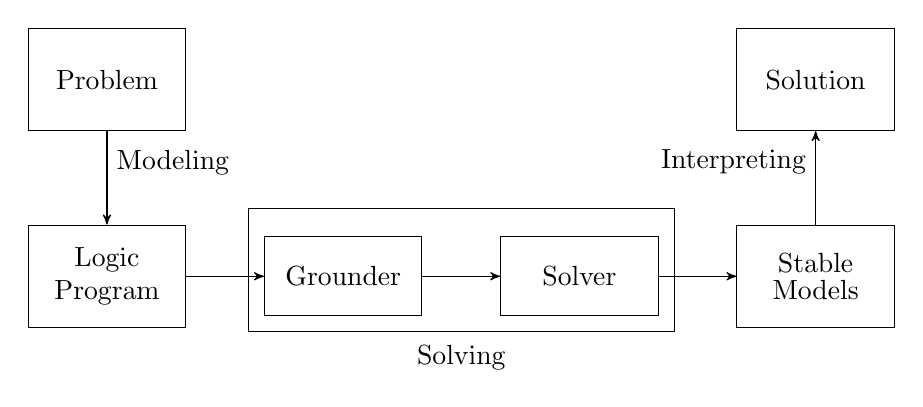
\begin{tikzpicture}[
      x=3cm,y=2.5cm,
      >=stealth',
      big box/.style={draw,minimum width=2cm,minimum height=1.3cm,inner sep=0},
      small box/.style={draw,minimum width=2cm,minimum height=1cm,inner sep=0},
      auto,
    ]
    \begin{scope}[every node/.style={big box}]
      \node (a) at (0,1) {Problem};
      \node (b) at (0,0) {\shortstack{Logic\\Program}};
      \node (e) at (3,0) {\shortstack{Stable\\Models}};
      \node (f) at (3,1) {Solution};
    \end{scope}
    \begin{scope}[every node/.style={small box}]
      \node (c) at (1,0) {Grounder};
      \node (d) at (2,0) {Solver};
    \end{scope}
    \node[above left, anchor=south west,inner sep=0,yshift=.1cm] (label) at (c.north west){\clingo};
    \node[draw,fit=(c) (d) (label),inner sep=.2cm] {};
    \path[->]
      (a) edge node [yshift=.2cm] {Modeling} (b)
      (b) edge (c)
      (c) edge node [swap,yshift=-.75cm] {Solving} (d)
      (d) edge (e)
      (e) edge node [yshift=.2cm] {Interpreting} (f);
  \end{tikzpicture}
  \caption{ASP solving process}%
  \label{fig:asp-in-a-nutshell}
\end{figure}

  The ASP solving process can be summarized by the steps depicted in \cref{fig:asp-in-a-nutshell}.
  \item \cite{cafascwa20a}
  \begin{itemize}
    \item Many real-world applications have a heterogeneous nature.
    Let it be in
    bio-informatics~\cite{frscscsiwa18a},
    hardware synthesis~\cite{newascha18b},
    or train scheduling~\cite{abjoossctowa19a},
    all cited ones consist of genuine qualitative and quantitative constraints.
    While the former often account for topological requirements, like reachability,
    the latter usually address (fine-grained) time or resource requirements.
    \item
    The hybrid nature of such applications has led to mixed solving technology,
    foremost in the area of Satisfiability modulo Theories (SMT;~\cite{niolti06a}).
    \item
    Meanwhile,
the need for hybridization has also prompted similar approaches in neighboring areas such as Answer Set Programming (ASP;~\cite{lifschitz08b}).
    \item
    When it comes to extending ASP with foreign reasoning methods,
the design often follows the algorithmic framework of SMT and leaves semantic aspects behind.
For instance, a popular approach is to combine ASP with Constraint Processing (CP;~\cite{dechter03a}),
also referred to as Constraint ASP (CASP;~\cite{lierler14a}).
This blends non-monotonic aspects of ASP with monotonic ones of CP but
fails to provide a homogeneous representational framework.
In particular, the knowledge representation capabilities of ASP, like defaults and aggregates, remain inapplicable to constraint variables.
    \item
    We addressed this in~\cite{cakaossc16a} by integrating ASP and CP in the uniform semantic framework called \emph{Here-and-There with constraints}~(\HTC).
    \item
This relies upon the logic of Here-and-There (\HT;~\cite{heyting30a}) along with
its non-monotonic extension, called Equilibrium Logic~\cite{pearce96a}.
    \item
    As an example,
consider the hybrid ASP rule%
\footnote{We put dots on top of braces, viz.~``$\agg{ \dotsc }$'', to indicate \emph{multisets}.}
\begin{gather}\label{eq:tax.sum}
  \mathit{total}(R) := \mathit{sum}\agg{ \, \mathit{tax}(P) : \mathit{lives}(P,R) \,  } \ \leftarrow \ \mathit{region}(R)
  \quad
\end{gather}
gathering the total tax revenue of each region $R$ by summing up the tax liabilities of the region's residents, $P$.
%
As a matter of fact,
the calculation of tax liability is highly complex, and relies on defaults and discounts to address incomplete information,
which nicely underlines the need for non-monotonic constraint variables.
  \end{itemize}
  \item \cite{cafascwa20b}
    \begin{itemize}
      \item 
      This integration is however often done in system-oriented ways that leave semantic aspects behind.
    \end{itemize}
\end{itemize}

\section{Selected contributions}

\section{Overall contributions}

\begin{itemize}
  \item list all my contributions + how others are using them
\end{itemize}

\begin{itemize}
  \item check the Promotionsordnung for requirements
  \item my papers: \cites{}
\end{itemize}

\chapter{Publications}\label{sec:publications}

This section contains selected publications.

\includepub{%
  title={Potassco: The Potsdam Answer Set Solving Collection},
  label={sec:publications:potassco},
  path={pub/potassco.pdf},
  authors={Martin Gebser, Benjamin Kaufmann, Roland Kaminski, Max Ostrowski, Torsten Schaub and Marius Schneider},
  published_in={AI Communications 24 (2011) 107–124},
  bibentry={\cite{gekakaosscsc11a}},
  doi={10.3233/AIC-2011-0491}}


\chapter{Discussion}\label{sec:discussion}



\chapter{Summary}\label{sec:summary}


\appendix

\backmatter
\bibliography{local,krr,procs}

\end{document}

%%% Local Variables:
%%% mode: latex
%%% TeX-master: t
%%% End:
